\subsection{Pileup Studies}
\label{sec:pileup_studies}

To study the effect of pileup on the UE measurement, the average pile up rates run-by-run is determined for full set of good runs during the Run 2024 p+p data taking period.
The run integrated MBD live rate is used to determine the average pile up rates as the live rate is directly related to the number of collisions seen by the sPHENIX detector.
The average pile up rate calculation assumes that simultaneous collisions are given by a Poisson distribution: $P(k) = (\lambda^{k}e^{-\lambda})/k!$ where $\lambda$ is the average number of collisions per bunch crossing.
Therefore, $\lambda$ can be calculated as $\lambda = f_{c}/(f_{b}*N)$ where $f_{c}$ is the run integrated MBD live rate, determined run-by-run by the number of MBD live counts divided by the length of the run in seconds, the bunch crossing rate is $f_{b} = 78 kHz$ and bunch number $N = 111$. 

The average pileup rate follows as:
\begin{equation}
   \langle PU \rangle = \frac{P(k>1)}{P(1)+P(k>1)}
\end{equation}
Here the average pileup rate is calculated from the triggered dataset; therefore this quantity can be understood as "given a crossing with a collision, what is the probability of that crossing having more than one collision".
The MBD live rates range run-by-run from 60kHz-2MHz across the full Run 2024 p+p dataset with the largest variation in the MBD live rates in the early period of the Run when the beam crossing angle at the sPHENIX interaction point was at 0 mrad. 
When the beam crossing angle at the sPHENIX IP was at 1.5mrad, later in p+p Run, the MBD live rates were lower overall and the variation across a store of runs was small. 
The full range of MBD live rates across the Run 2024 p+p dataset correspond to run-by-run average pile up values from $< 1\%$ to $> 10\%$. 
The average pileup value and MBD live rate for each run are shown in Figure~\ref{fig:pileup_runbyrun}. 
Here a clear difference in the average pileup rate and MBD live rate can be seen for the two different beam crossing angles, with a switch in crossing angle occuring just after run number 51000.

\begin{figure}
    \centering
    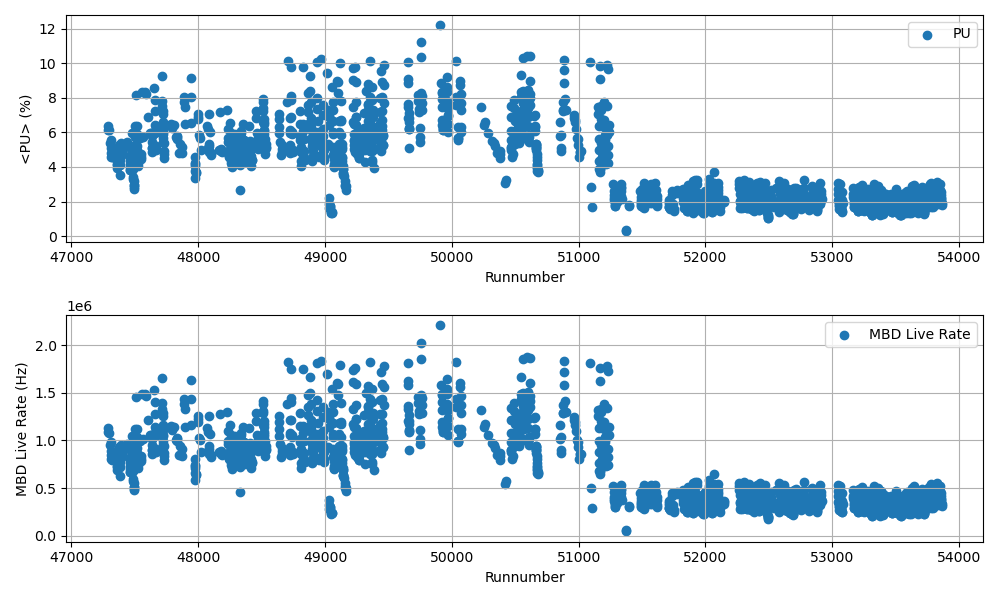
\includegraphics[width=\linewidth]{ueinpp/Figures/pileup/run_by_run_pileup.png}
    \caption{Run-by-run average pileup (top) and MBD live rate (bottom) for the full Run 2024 p+p dataset.}
    \label{fig:pileup_runbyrun}
\end{figure}

For this study, nine pile up ranges are used to determine the level of pileup effects on the UE measurement.
These ranges are $\langle PU\rangle < 2\%$, $2\% < \langle PU\rangle < 3\%$, $3\% < \langle PU\rangle < 4\%$,
 $4\% < \langle PU\rangle < 5\%$, $5\% < \langle PU\rangle < 6\%$, $6\% < \langle PU\rangle < 7\%$, 
 $7\% < \langle PU\rangle < 8\%$, $8\% < \langle PU\rangle < 9\%$, $9\% < \langle PU\rangle < 10\%$.
 Values above 10\% are not included in this study.
The histogram of runs as a function of average pileup for the full dataset is shown in Figure~\ref{fig:avg_pileup}.

\begin{figure}
    \centering
    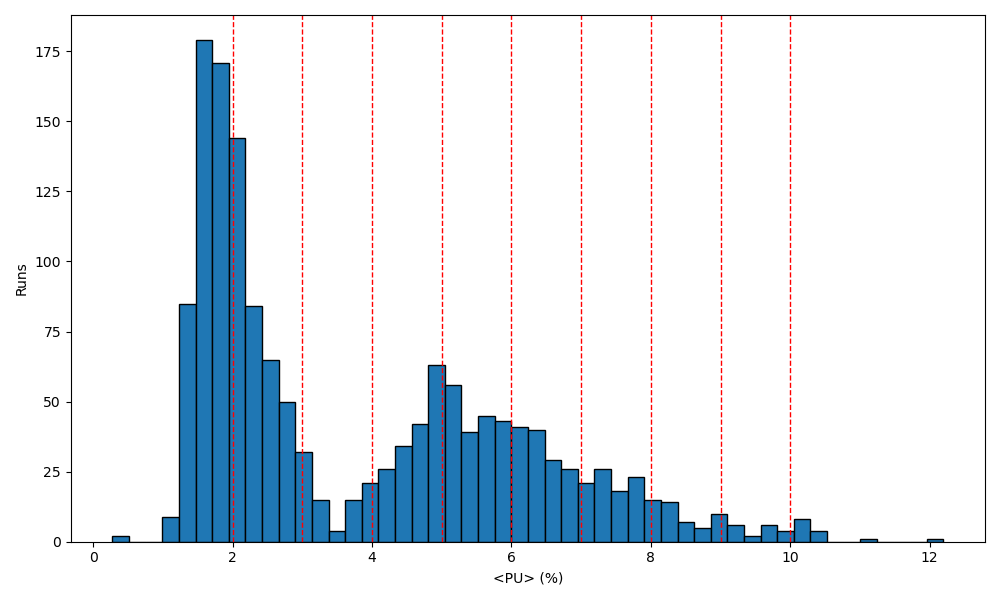
\includegraphics[width=0.7\linewidth]{ueinpp/Figures/pileup/avg_pileup.png}
    \caption{Histogram of runs as a function of average pileup for full Run 2024 p+p dataset.}
    \label{fig:avg_pileup}
\end{figure}

The UE measurement is then studied as a function of pileup using these average pileup bins. This study is conducted both using the full dataset and by investigating the two beam crossing angle datasets separately. 
The average $\Sigma E_T$ is calculated for each pileup range and a linear fit is performed to the average $\Sigma E_T$ for each pileup range for the full Run 2024 p+p dataset.
The slope of the linear fit is then used to determine the effect of pileup on the UE measurement.
The average $\Sigma E_T$ as a function of pile up and the linear fit are shown in Figure~\ref{fig:pileup_0mrad_1.5mrad_separately_together}.

The full dataset agrees fairly well with the linear fit indicating that the effect on the transverse region $\Sigma E_T$ can be described by a linear function on $\langle PU \rangle$
and a simple subtraction of the linear fit from the average $\Sigma E_T$ can be used to correct for the pileup effect.
There are some small deviations from the linear fit at high pileup which are expected as the MBD trigger becomes non-linear at high pileup.
However for this analysis only runs with average pileup $<6\%$ are included in the final measurement, therefore this non-linearity correction at high pileup does not affect the final measurement.
Additionally, the separate 0 mrad and 1.5 mrad beam crossing angle datasets agree well in the region they overlap, indicating that the pileup effect on the UE measurement can be treated in a similar manner for these two different beam crossing angle setups.

\begin{figure}
    \centering
    \begin{subfigure}[t]{0.48\linewidth}
        
\includegraphics[width=\linewidth]{{ueinpp/Figures/pileup/pileup_0mrad_1.5mrad_separately}.png}
        \caption{Average $\Sigma E_T$ density for 0 mrad crossing angle dataset (open) and 1.5 mrad crossing angle dataset (closed)}
    \end{subfigure}
    \hfill
    \begin{subfigure}[t]{0.48\linewidth}
        
\includegraphics[width=\linewidth]{{ueinpp/Figures/pileup/pileup_0mrad_1.5mrad_together_dijet_w_bkgcuts}.png}
        \caption{Average $\Sigma E_T$ for the full Run 2024 p+p dataset (closed)}
    \end{subfigure}
    \caption{Average $\Sigma E_T$ density and $\Sigma E_T$ as a function of pileup for the separate beam crossing angle datasets, 0 mrad (open) + 1.5 mrad (closed), (left) and for the full Run 2024 p+p dataset (right). A linear fit to the average $\Sigma E_T$ (black line) is included for the full dataset case.}
    \label{fig:pileup_0mrad_1.5mrad_separately_together}
\end{figure}

\subsection{Pileup Application}
\label{sec:pileup_application}

Pileup effects are studied by examining the relationship between the average pileup, determined on a run-by-run basis, and the transverse region average total $E_{T}$. 
A pileup correction, derived from the slope of the linear fit to the transverse region average total $E_{T}$ of clean dijet events passing the cuts outlined in Section~\ref{sec:ueinpp_jetbackground} shown in Figure~\ref{fig:pileup_0mrad_1.5mrad_separately_together}, is applied to the reconstructed transverse region $E_{T}$ prior to unfolding. 
Pileup corrections derived from clean inclusive jet events, jets passing the cuts outlined in Section~\ref{sec:ueinpp_jetbackground}, namely the energy fraction cut and timing cuts, were also derived and found to be consistent with the pileup correction derived from clean dijet events.

Figure~\ref{fig:pu_reco_unfolded} compares reconstructed and unfolded distributions with and without the pileup correction. 
Small differences are observed in the $E_{T}$ distribution at the reconstructed level and the effect on the mean of the reconstructed $E_{T}$ distribution shown in the legends of Figure~\ref{fig:pu_reco_unfolded} is also relatively small.
The effect on the unfolded mean transverse region $E_{T}$ is $<4\%$ for all leading jet $p_{T}$ bins in the measurement range.  

As a result, the final measurement uses the results with the pileup correction applied and as a systematic uncertainty on the effect of pileup this pileup correction is toggled off.
The observed difference between the pileup correction on and off is treated as a systematic uncertainty, shown for an unfolded distribution in Figure~\ref{fig:pu_reco_unfolded}, and is found to have at most a $4\%$ effect on both the reconstructed and unfolded average transverse region $E_{T}$.
 
\begin{figure}
    \centering
    \begin{subfigure}[t]{0.48\linewidth}
        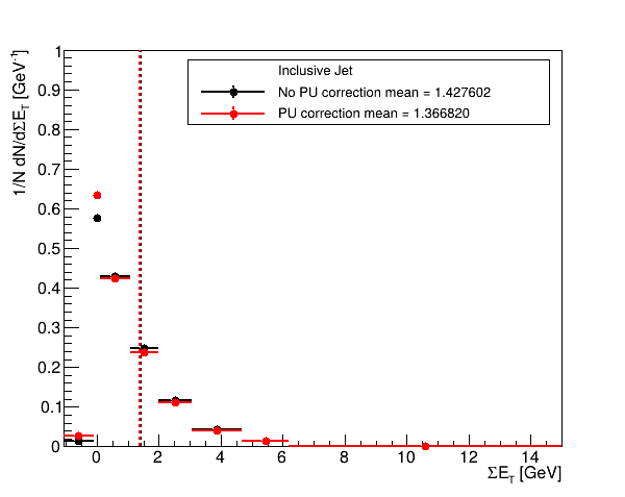
\includegraphics[width=\linewidth]{ueinpp/Figures/pileup/pileup_effects_reco_inclusive.png}
        \caption{Reconstructed transverse region $E_{T}$ distribution for inclusive jet events with and without pileup correction.}
    \end{subfigure}
    \hfill
    \begin{subfigure}[t]{0.48\linewidth}
        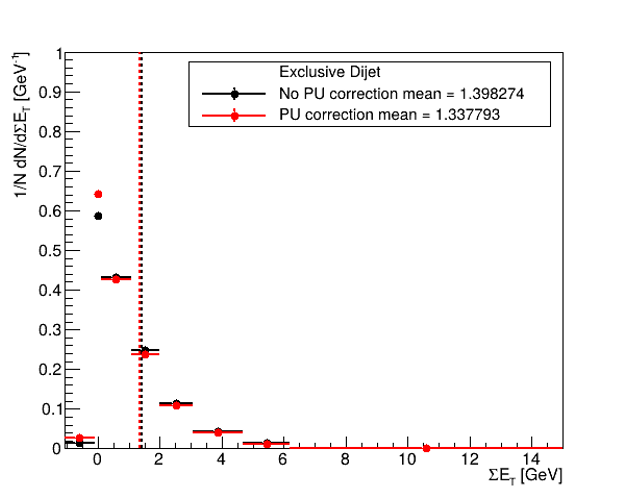
\includegraphics[width=\linewidth]{ueinpp/Figures/pileup/pileup_effects_reco_dijet.png}
        \caption{Reconstructed transverse region $E_{T}$ distribution for dijet events with and without pileup correction.}
    \end{subfigure}
    \begin{subfigure}[t]{0.48\linewidth}
        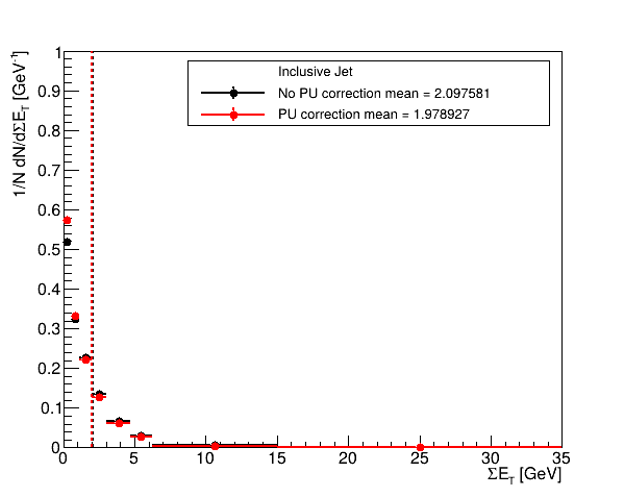
\includegraphics[width=\linewidth]{ueinpp/Figures/pileup/pileup_effects_unfolded_inclusive.png}
        \caption{Unfolded transverse region $E_{T}$ distribution for inclusive jet events with and without pileup correction.}
    \end{subfigure}
    \hfill
    \begin{subfigure}[t]{0.48\linewidth}
        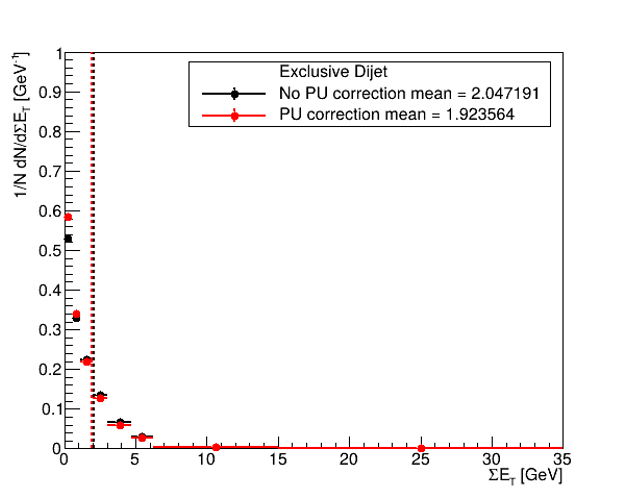
\includegraphics[width=\linewidth]{ueinpp/Figures/pileup/pileup_effects_unfolded_dijet.png}
        \caption{Unfolded transverse region $E_{T}$ distribution for dijet events with and without pileup correction.}
    \end{subfigure}
    \caption{Reconstructed (top) and unfolded (bottom) transverse region $E_{T}$ distributions for inclusive jet (left) and dijet (right) events with and without the pileup correction.}
    \label{fig:pu_reco_unfolded}
\end{figure}